\documentclass[10pt, twocolumn]{IEEEtran}
% Leaving this next line in to periodically check how many Normal People Pages were written
%\documentclass[12pt, letterpaper]{article}
\usepackage[utf8]{inputenc}

\usepackage{listings}
\usepackage{xcolor, color, soul}
\usepackage{multirow}
\usepackage{tabulary}

\definecolor{codegreen}{rgb}{0,0.6,0}
\definecolor{codegray}{rgb}{0.5,0.5,0.5}
\definecolor{codepurple}{rgb}{0.58,0,0.82}
\definecolor{backcolour}{rgb}{0.95,0.95,0.92}

\lstset{
	language=c++,
	backgroundcolor=\color{backcolour},   
	commentstyle=\color{codegreen},
	keywordstyle=\color{magenta},
	numberstyle=\tiny\color{codegray},
	stringstyle=\color{codepurple},
	basicstyle=\ttfamily\footnotesize,
	breakatwhitespace=false,         
	breaklines=true,                 
	captionpos=b,                    
	keepspaces=true,                 
	numbers=left,                    
	numbersep=5pt,                  
	showspaces=false,                
	showstringspaces=false,
	showtabs=false,                  
	tabsize=2
}

\usepackage{graphicx}
\usepackage{mathtools}

\usepackage[style=apa, backend=biber]{biblatex}
\addbibresource{paper.bib}

\title{Granular Synthesis for Instrument Makers}
\author{	
	\IEEEauthorblockN{Daniël Kamp\\}
    \IEEEauthorblockA{HKU University of the Arts Utrecht
    \\Department of Music and Technology
    \\daniel.kamp@student.hku.nl}
    }
\date{May 2022}

\begin{document}

\maketitle

\begin{abstract}
This writing sheds light onto various forms of granular synthesis. It analyses some existing applications, explains the inner workings of such systems, and proposes methods of how one may implement the technique themselves.
\end{abstract}

\section*{Introduction}
Granular synthesis is a versatile form of sample-based (digital) sound synthesis. It uses short slices of recorded audio to create new, rich sounds. These slices can be layered, stretched, spread, and in other ways processed to create vast soundscapes with relative ease. \\
This writing aims to demystify the technical aspects of granular synthesis, and provide a comprehensive insight for instrument makers who want to make use of the technique.

\section{What is granular synthesis?}
This first part tells a brief history of granular synthesis, explains the components of a system implementing this technique, and lists some reference instruments.

\subsection{A brief history}
Granular synthesis as it's known today is a form of digital sound synthesis, which is based on the processing of small slices of sampled audio known as "grains". The underlying view on sound perception was first proposed by Hungarian-British physicist Dennis Gabor in an article titled \textit{Acoustical Quanta and the Theory of Hearing} (\cite{gabor47}). In this writing, Gabor theorized an approach to sound similar to concepts found in quantum mechanics.\\ Building on this theory, in the late 1950s, Greek composer Iannis Xenakis started experimenting with the technique, stitching together many tiny slices of tape to create new sounds (\cite{robindore96}). Inspired by Xenakis during a 1972 workshop taught by the former, composer Curtis Roads eventually created the first computer software implementing this synthesis paradigm in 1974 (\cite{opie03}). His code produced a 30-second long piece titled Klang-1, using three parameters: envelope, duration, and density. This software, however, did not operate in real-time, and producing this piece of music took multiple days. The first real-time implementation of the principle came from Canadian composer Barry Truax, who developed GSX (1986) and GSAMX (1987) (\cite{truax88}). \\
Since then, granular synthesis has established itself as a pillar of modern digital sound generation. More approachable implementations of the technique, like Robert Henke's Granulator (2011), made it possible for anyone with a computer to explore its vast new possibilities in sound. Today, dozens of granular synthesizers are available, each offering a different approach to a 75-year-old concept.

\subsection{General system overview}
This section describes the general anatomy of a granular synthesizer, and gives a broad overview of the building blocks that make up such a system. 

\begin{figure}[ht!]
	\centering
	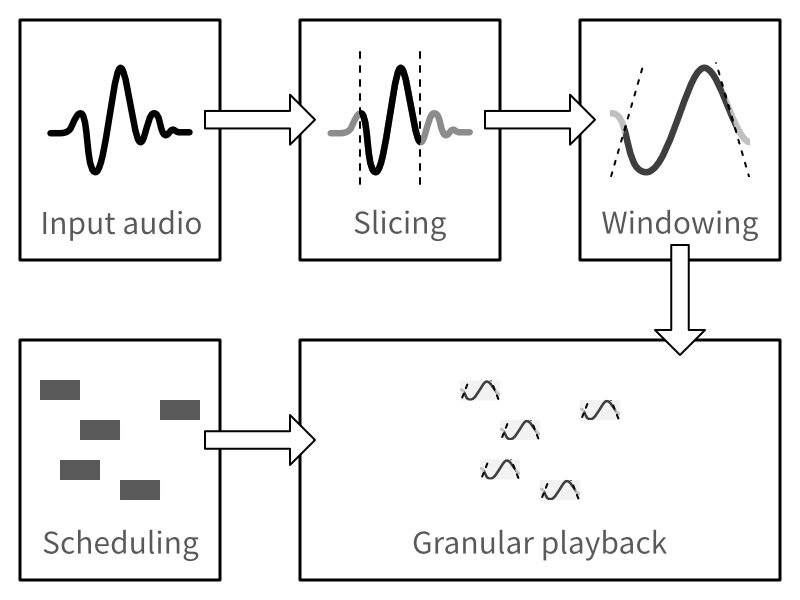
\includegraphics[width=0.75\linewidth]{GranularDiagram.png}
	\caption{A simplified overview of a granular synthesis system.}
	\label{fig:block_diagram}
\end{figure}

\subsubsection{Sound source}
As its input, a granular system takes a sound stream. This stream can consist of sampled audio, live microphone input, or generated audio (such as sine waves). The content of this source material has an effect on the sounds one can generate: when using a transient-rich source, for example a drum sample, the resulting audio will usually have a substantial amount of content in the higher regions of the frequency spectrum. Sounds with a more periodic envelope are more suitable for generating melodic content, since they usually result in a more mellow output sound.\\

\subsubsection{Models}
There are four distinguishable models of granular synthesis: screen, cloud, stream, and spray (\cite{roads12}). The first of these, screen, was described by Xenakis and would run a series of time-frequency plots at a fixed time rate (\cite{xenakis63}). In layman's terms, this would be comparable to a flip book animation, used for sound instead. \\
The second model, clouds, generates a cloud of sound in which the individual grains are not bound to predefined parameters, but instead spread across specified ranges in a stochastic manner. This creates rich, unpredictable textures that are often used on a macro level within compositions. \\
The more regular counterpart of clouds is streams, in which grains are distributed in a deterministic process. In this model, the density (number of grains per second) determines a regular interval at which grains are played, creating a sort of rhythmic texture. This rhythm can be tweaked by modifying the grain density, through which one can create tone-like sounds. \\
A model that is used in modern digital granular synthesis is spray. This implementation makes it possible for users to draw the grains on a plot of frequency over time, which makes for an intuitive interaction model.\\

\subsubsection{Windowing and envelope}
Since the start position of grains is rather arbitrary, there is no telling what the amplitude of the first sample in the selection will be. Therefore, it's good practice, as it is in any digital audio application, to apply an envelope that trims off any rough edges that may exist in the source material. This envelope can be modified to a user's own insight through the parameters \textit{shape} and \textit{length}. \\
The shape of an envelope refers to its mathematical function. In this regard, there are four commonly used shapes: linear, square root, exponential, and Gaussian. The latter was proposed by Dennis Gabor in his original theory on granular sound, and is still commonly used. More recently, due to developments in the field of processing power in computers over the past fifty-or-so years, it has become possible and commonplace to use other envelope shapes as well. Figure \ref{fig:env_shapes} shows the four functions as a plot of amplitude over time.

\begin{figure}[ht!]
	\centering
	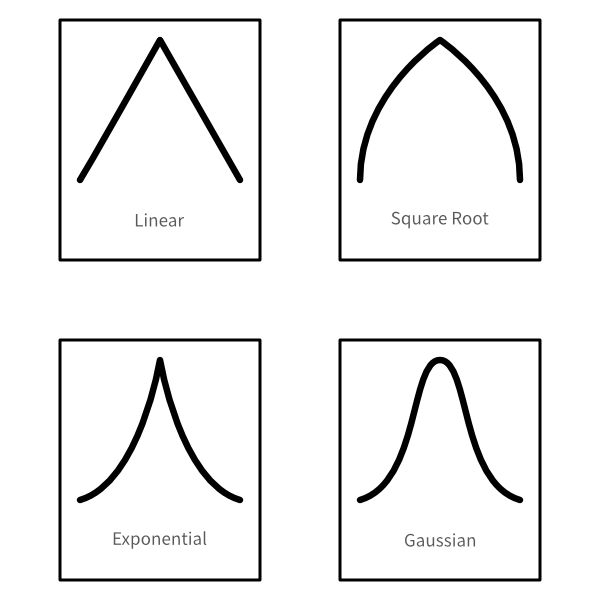
\includegraphics[width=0.5\linewidth]{env_shapes.png}
	\caption{Four envelope shapes.}
	\label{fig:env_shapes}
\end{figure}

The length of an envelope simply describes the time it takes for the signal to reach its full amplitude. By varying this number, one can change the character of the resulting sound. If a long \textit{attack} (rising edge of the envelope) is used, the resulting audio will sound more mellow compared to when a short attack time is applied.\\

\subsubsection{Duration and density}
Density, as mentioned previously, describes the number of grains played in one (1) second. Variations in this domain can roughly be split into two categories: \textit{deterministic} and \textit{stochastic}.\\
In a deterministic distribution, grains are played back with even spacing between them. This means that the resulting sound is of a regular nature. For example, this method would produce audio in which a grain is played every 100 ms. \\
Stochastic distribution, on the other hand, adds a realm of uncertainty to the sound. When this distribution is applied, the beginning and length of each grain are randomized. This means that the resulting sound is no longer predictable and/or regular in nature. Using this method, one can create vast clouds of sound that contain no structure or repetition.

\subsection{Existing instruments}
This section lists a few instruments and effects that use granular synthesis. \\
\textit{Author's note:} I selected open-source instruments of which the source code is freely available to the public. This way, I can give an in-depth comparison of the inner workings of these instruments. I'll use these and their concrete implementations as references throughout the rest of my research described in this writing.\\

\subsubsection{Mutable Instruments' Clouds}
Clouds is a Eurorack module developed and produced by Émilie Gillet (Mutable Instruments). Both the hardware files (schematics, CAD-files) and firmware source code are open-source and publicly available (\cite{clouds}).\\
As its source sound, Clouds uses incoming stereo audio compliant with the Eurorack standard.\\
Looking at the source files of Clouds, one can dissect the process used to "seed" grains. First, a maximum number of grains is "hard-coded" into the software. The program will create new ones until this limit is reached. Clouds offers both deterministic and stochastic seeding modes, which can be selected by the user. In deterministic mode, one controls the time between seeds in a regular manner. In stochastic mode, the user input controls the likelihood with which grains will be created.\\
This implementation uses so-called Look Up Tables (LUTs) to store data for its envelopes and other resource-intensive processes. These tables contain pre-calculated numbers, so that the program doesn't need to calculate these in real-time. This makes it suitable for low-power devices (in case of Clouds, this is an STM32 micro-controller). The next chapter contains examples of, and a comparison between this implementation and one that does calculate its data in real-time.\\

\subsubsection{Argotlunar}
Argotlunar is a real-time granular VST and AudioUnit plugin created by Michael Ourednik. The source code of this software is open-source and available via GitHub (\cite{argotlunar}). This granular effect is implemented using the JUCE framework.

Since Argotlunar is designed to run as a plug-in within a Digital Audio Workstation, it will usually have more computing resources available than the previous example. This is apparent in its code, as liberties have been taken that would probably be avoided on embedded systems. For example, a lot of the variables that are needed during sound processing are generated at runtime. In low-power systems, it's common practice to avoid this by calculating the data beforehand and compiling them into the program.

\section{How does granular synthesis work?}
This part dives deeper into the inner workings of a granular system. Starting with a brief explanation of core audiological concepts that define how we experience sound on a short time scale, it then proceeds to explain concrete implementations of a granular synthesizer in C++. These examples are then compared through statistics about their performance, so a recommendation can be made based on system efficiency.

\subsection{Audiological concepts}
The granular synthesis technique relies heavily on the psycho-acoustical concept of \textit{forward masking} (\cite{bates04}). This "limitation" of human perception causes sound impulses at quick succession to blend together and be perceived as a continuous tone. In numbers, a threshold for this interval between two impulses can be established at around 10ms (\cite{gabor47}), which corresponds to a frequency of 100Hz. However, if succeeding impulses are played at half the intensity of that first impulse, the time between sounds can be as long as 21ms. In other words, if a short sound is played every 10-21ms, a human listener will perceive this as a continuous sound, and may even discern a (musical) tone.

\subsection{Runtime constraints}
The information above, however, only applies in part to the digital world. Instead of generating sound in real-time, a computer uses an audio engine that renders its output in blocks. This system is capable of rendering a number of cycles at once. These are then scheduled by a separate process, allowing sound generation and playback to operate independently. This gives the rendering process more time to perform its calculations.

One such audio engine is the JACK Audio Connection Kit, a cross-platform toolkit for building and running audio applications. Using this program as an example, it's possible to calculate the constraints within which an implementation needs to operate.\\
In the author's setup, JACK has a default sample rate of 44.1kHz, and operates with a block size of 1024 frames per period. With this information, the time per block can be calculated as follows:
\[
	\textit{rendering time} = \frac{\textit{block size}}{\textit{sample rate}}
\]
This returns a rendering interval of around 23ms per block. Dividing it by the number of samples that need to be rendered during this time, the rendering time per cycle comes down to about 22$\mu$s. For simplicity, one may assume that this entire rendering time is available to the granular synthesis process.

\subsection{Implementations}
In this section, implementations and methods are proposed for specific parts of a granular system. The next section will take execution metrics from these example implementations, and validate them by the requirements defined previously.\\

\subsubsection{Scheduling algorithms}
This section gives four examples of grain scheduling algorithms, using two different approaches. These algorithms determine when grains are played, and thus heavily influence the resulting sound's character.\\

\textbf{Deterministic approach}\\
For a deterministic method, a user directly or indirectly controls the sound's \textit{density}, using parameters like \textit{grain length} and \textit{grain interval}. Playing back grains with a regular interval creates a predictable and periodic output sound, which can even be used in a melodic way. The following code example implements a deterministic approach for a single stream of grains.\\
\begin{minipage}{\linewidth}
\begin{lstlisting}[caption={A deterministic method of grain "seeding"}]
	int interval = grain_size / density;
	for (int i = 0; i < (block_size - interval); i += interval) {
		grains.push_back(Grain(i));
	}
\end{lstlisting}
\end{minipage}

\textbf{Stochastic implementation 1: random start position}\\
To add variation to a sound, one might want to depart from a periodic triggering algorithm like the one described above. The cloud model, as mentioned in section 1.B, exchanges the regular interval for random chance. \\
This first implementation uses randomness to determine the starting position of each grain. To generate its random numbers, it uses C++'s built-in \lstinline|std::rand()| function.
\begin{minipage}{\linewidth}
\begin{lstlisting}[caption={A stochastic method of grain seeding: random start position}]
	int max_grains = floor(MAX_GRAINS * spawn_likelihood);
	for(int i = 0; i < max_grains; i++) {
		float v = (float) rand() / (float) RAND_MAX;
		grains.push_back(Grain((int) (block_size * v)));
	}
\end{lstlisting}
\end{minipage}

\textbf{Stochastic implementation 2: random chance}\\
This second stochastic method loops through the rendering block and uses randomness to determine whether a grain is to be scheduled on the current position. It includes a minimum offset between grains, so that a high percentage of the block is guaranteed to be covered. Additionally, it swaps the built-in \lstinline|std::rand()| function for the \lstinline|<random>| library that is included with the C++ Standard Library.
\begin{minipage}{\linewidth}
\begin{lstlisting}[caption={A stochastic method of grain seeding, using \lstinline|<random>|}]]
	random_device rd;
	mt19937 gen(rd());
	uniform_real_distribution<> dist(0, 1);
	int wait = 0;

	for(int i = 0; i < block_size; i++) {
		if(wait == 0) {
			v = dist(gen);
			seed = v < spawn_likelihood;
			if(max_grains > 0 && seed) {
				grains.push_back(Grain(i));
				max_grains--;
				wait = minimum_interval;
			}
		} else {
			wait--;
		}
	}
\end{lstlisting}
\end{minipage}

\textbf{Combined approach: Divide-down}\\
To add rhythm to the chaos of using a stochastic approach, one might add a deterministic element. Figure \ref{fig:divide_down} shows how a combination of these two implementations might look. In this example, each grain has a random chance to be seeded. \\ 
\begin{figure}[ht!]
	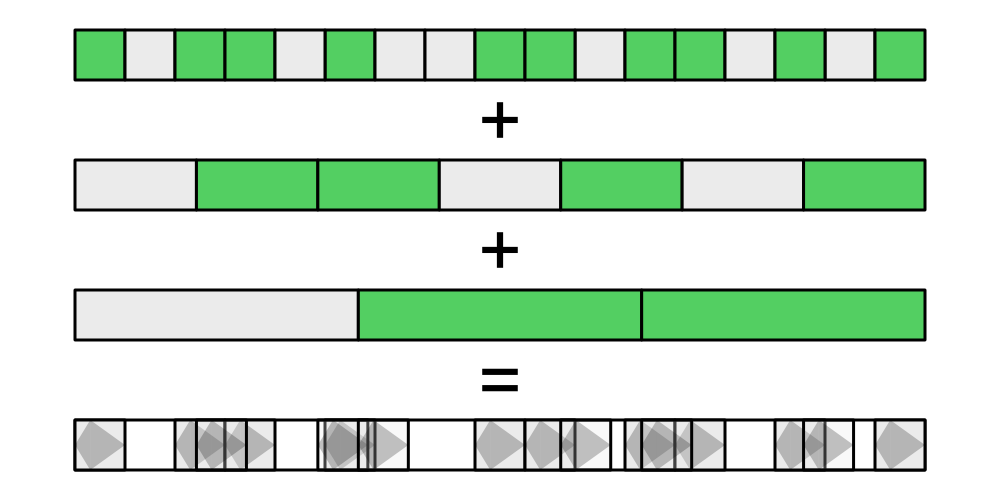
\includegraphics[width=\linewidth]{divide_down.png}
	\caption{A divide-down algorithm visualized.}
	\label{fig:divide_down}
\end{figure}

During each loop, the full length of the rendering block is divided by the remaining number of grains. By layering these divisions, one can create a cloud of unpredictable sound, while still retaining a certain structure.

The following code combines the examples from \textbf{Deterministic approach} and \textbf{Stochastic approach 2}.\\
\begin{minipage}{\linewidth}
\begin{lstlisting}[caption={An implementation of a divide-down algorithm}]
	int max_grains = 64;
	int number_of_grains = 0;	
	int interval = (float) block_size / (float) max_grains;

	while(max_grains > 1) {
		interval = (float) block_size / (float) max_grains;
		
		if(interval > minimum_interval) {
			for (int i = 0; i < (block_size - interval); i += interval) {
				if(max_grains > 0) {
					v = dist(gen);
					seed = v > spawn_likelihood;
					if (seed) {
						grains.push_back(Grain(i));
						max_grains--;
					}
				}
			}
		} else {
			max_grains = 0;
		}
	}
\end{lstlisting}
\end{minipage}\\

\subsubsection{Windowing algorithms and approaches}
This section compares three approaches for implementing an envelope generator. For simplicity, each method renders a quadratic parabola envelope shape with a duration of 4096 samples.  \\

\textbf{First implementation: Pre-rendering}\\
This method calculates a new lookup table when any values (such as envelope or grain length) are changed. This way, the program can simply look up and apply the right value during the rendering process, without needing additional calculations.\\
\begin{minipage}{\linewidth}
\begin{lstlisting}[caption={Envelope application using a pre-rendering algorithm}]
	#define ENV_ROUNDS 4096
		
	float envelope[ENV_ROUNDS];
	float intermediate_;
		
	// Initialization, runs once
	for(int i = 0; i < ENV_ROUNDS; i++) {
		intermediate_ = ENV_SHAPE * (float)(-1.0 * i * i + ENV_ROUNDS * i);
		envelope[i] = (intermediate_ >= 1.0) * 1.0 + (intermediate_ < 1.0) * intermediate_;
	}
		
	// Rendering loop, runs while active
	for(int i = 0; i < ENV_ROUNDS; i++) {
		test1[i] = sample[i] * envelope[i];
	}
\end{lstlisting}
\end{minipage}

\textbf{Second implementation: Look-Up Table}\\
In this next example, the program first scales its position in relation to the generated look-up table. Using this scaled position, it looks up the nearest corresponding value. It then uses a low pass filter to interpolate between the current and previous value.\\
The following formula was used to generate the data for the look-up table:
\[
y_n(x_n) = \frac{0.001*((\text{-}x_n^2)+\textit{grain size}*x_n)}{\textit{grain size}}
\]
\[	
f_n(y_n) = \frac{3}{2} * \begin{cases}
	\frac{y_n^3}{3}  	& y_n < 1.0 \\
	\frac{2}{3} 	& y_n \geq 1.0
\end{cases}
\]
\begin{minipage}{\linewidth}
\begin{lstlisting}[caption={Envelope application using a look-up table}]
	// Initialization, runs once
	float ENVELOPE_LUT[6000] = {0, 0.00149975, 0.002998996, 0.004497737, ...};
	
	auto scale_factor = (sizeof(ENVELOPE_LUT) / sizeof(ENVELOPE_LUT[0])) / ENV_ROUNDS;
	float previous = ENVELOPE_LUT[0];
	int ptr = 0;
	float tmp = 0.0;
	
	// Rendering loop, runs while active
	for(int i = 0; i < ENV_ROUNDS; i++) {
		ptr = floor(scale_factor * i);
		
		tmp = 0.5 * (envelope[ptr] + previous);
		test2[i] = tmp * sample[i];
		
		previous = envelope[ptr];
	}
\end{lstlisting}
\end{minipage}

\textbf{Third implementation: Real-Time Rendering}\\
This last example is taken directly from the Argotlunar source code. It calculates a step and slope value, and uses these to increment the envelope's multiplication variable.\\
\begin{minipage}{\linewidth}
\begin{lstlisting}[caption={Envelope application using real-time rendering}]
	// Code by M. Ourednik
	// Initialization, runs once
	float env_amp = 0.0f;
	float d = 1.0f / ENV_ROUNDS;
	float d2 = d * d;
	float slope = 4.0f * 0.8 * (d - d2);
	float curve = -8.0f * 0.8 * d2;
	
	// Rendering loop, runs while active
	for (int i = 0; i < ENV_ROUNDS; i++) {
		env_amp += slope;
		slope += curve;
		test3[i] = sample[i] * env_amp;
	}
\end{lstlisting}
\end{minipage}


\subsection{Efficiency}
For this section, the implementations from above were ran multiple times, to gain an accurate result. The execution time of each loop iteration has been recorded, along with the initialization time. Note that these benchmarks were ran on a 2019 MacBook Pro (Intel Core i7 6-core processor, 16GB RAM).

\subsubsection{Scheduling algorithms}
The first results describe the performance of the scheduling algorithms proposed earlier. These implementations are compared not by execution time necessarily, but more so by adherence to a user's intention. For example, if a user turns the density knob, the resulting sound should reflect the desired changes.\\
\begin{figure}[ht!]
	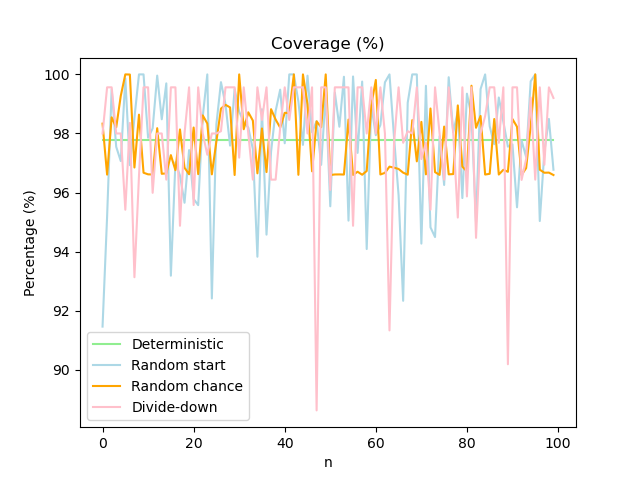
\includegraphics[width=\linewidth]{scd_coverage.png}
	\caption{Percentage of the rendering block covered by each algorithm, measured 100 times.}
	\label{fig:scd_coverage}
\end{figure}

This coverage analysis shows that all methods spread the grains evenly over the entire block. A deterministic approach always ensures the same coverage, which is to be expected when all parameters stay the same. Out of the stochastic methods, the divide-down algorithm shows the most variation in density between blocks. The other two stochastic algorithms perform rather similar.\\
\pagebreak

In the next test, the linearity between user input and the density of the output were measured. This was done by increasing the input value with $ \frac{1}{100} $ over 100 total measurements.
\begin{figure}[ht!]
	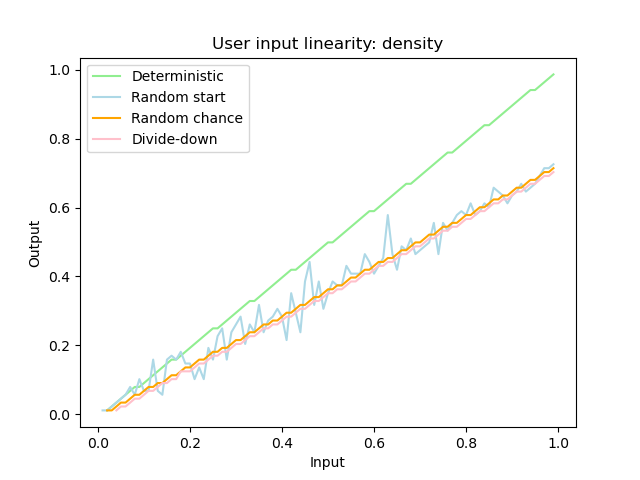
\includegraphics[width=\linewidth]{scd_linearity.png}
	\caption{Correlation between user input and system output. Measured on the interval $ \textit{input} =[0,1] $.}
	\label{fig:scd_linearity}
\end{figure}

These results show a direct correlation between the user's input and the system's output density. As to what causes the difference in slope: this is currently unknown, and requires further investigation. The author believes it to be a result of the relation between grain size and interval.\\

In this next analysis, the execution time per cycle was measured for each of the four different implementations.
\begin{figure}[ht!]
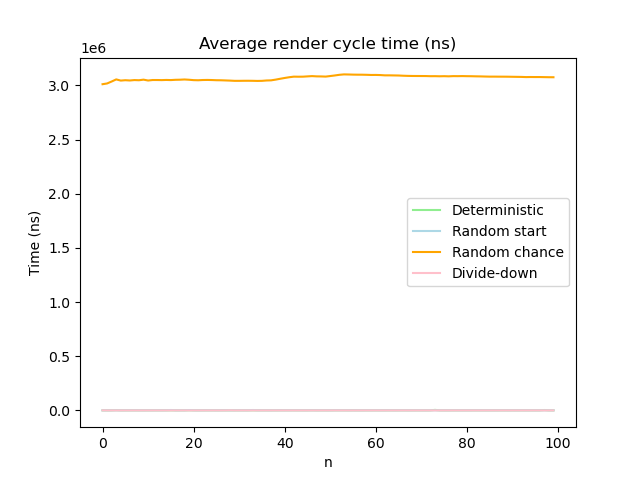
\includegraphics[width=\linewidth]{scd_cycle_time.png}
\caption{Average time per scheduling rendering cycle, measured 100 times.}
\label{fig:scd_cycle_time}
\end{figure}

The obvious takeaway from this data is that the \textit{random chance} algorithm takes extremely long to complete its rendering. In the graph, this makes it impossible to analyze the other data. When leaving out this method, one can get a better picture of the performance of these other implementations. This detailed view is pictured in Figure \ref{fig:scd_cycle_time_detail}.\pagebreak
\begin{figure}[ht!]
	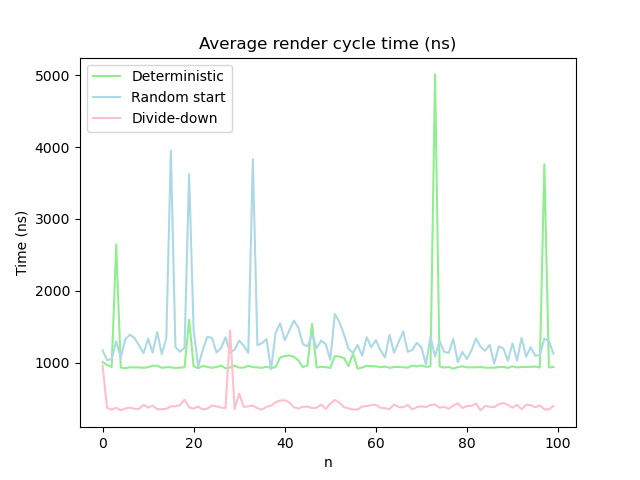
\includegraphics[width=\linewidth]{scd_cycle_time_detail.png}
	\caption{Average time per scheduling rendering cycle, measured 100 times, without \textit{random chance}.}
	\label{fig:scd_cycle_time_detail}
\end{figure}

This graph shows comparable performance for the \textit{random start} and \textit{divide down} approaches. They both have irregular execution time, which is to be expected when using random variables. The latter, however, takes slightly longer to process, likely due to its reliance on recursion. Still, the two algorithms perform similarly enough to be considered interchangeable.\\
Next, the \textit{deterministic} approach stands out due to its extremely short processing time. This is likely due to the fact that this method uses a far shorter loop than all other implementations. Instead of stopping at each sample in the block, it increments its position by a calculated interval. Because of this implementation, the loop has less code to execute, and thus takes significantly less time.

Keeping in mind the maximum rendering time of 23$\mu$s, as calculated previously, it's clear that the \textit{random chance} algorithm, with an average rendering time of 203$\mu$s, does not meet the criteria. Comparing the other three outcomes, with averages of 843ns, 1.1$\mu$s, and 1.7$\mu$s respectively, one would likely choose to implement a method with a low rendering time. However, it must be noted that all three algorithms have varying use-cases and render different results. While the \textit{deterministic} method might have a short execution time, its output may be too repetitive for some applications. Nevertheless, as a product solely of these statistics, it's unlikely that any of the three remaining approaches would offer insufficient performance for most applications.\\

\subsubsection{Envelopes}
Next, the benchmark results of the envelope implementations show some interesting details. Before looking at the runtime statistics, let's analyze the initialization times of each algorithm. Figure \ref{fig:env_init_time} shows this data, measured in nanoseconds. Looking at this graph, one will notice that the pre-processing implementation takes significantly longer to initialize than its counterparts. This can be attributed to the way this method renders its data all at once during this initialization phase. However, this probably won't affect the program's execution, as the initialization code is only ran sporadically and does not need to fit within the 23$\mu$s rendering time constraint.\pagebreak
\begin{figure}[ht!]
	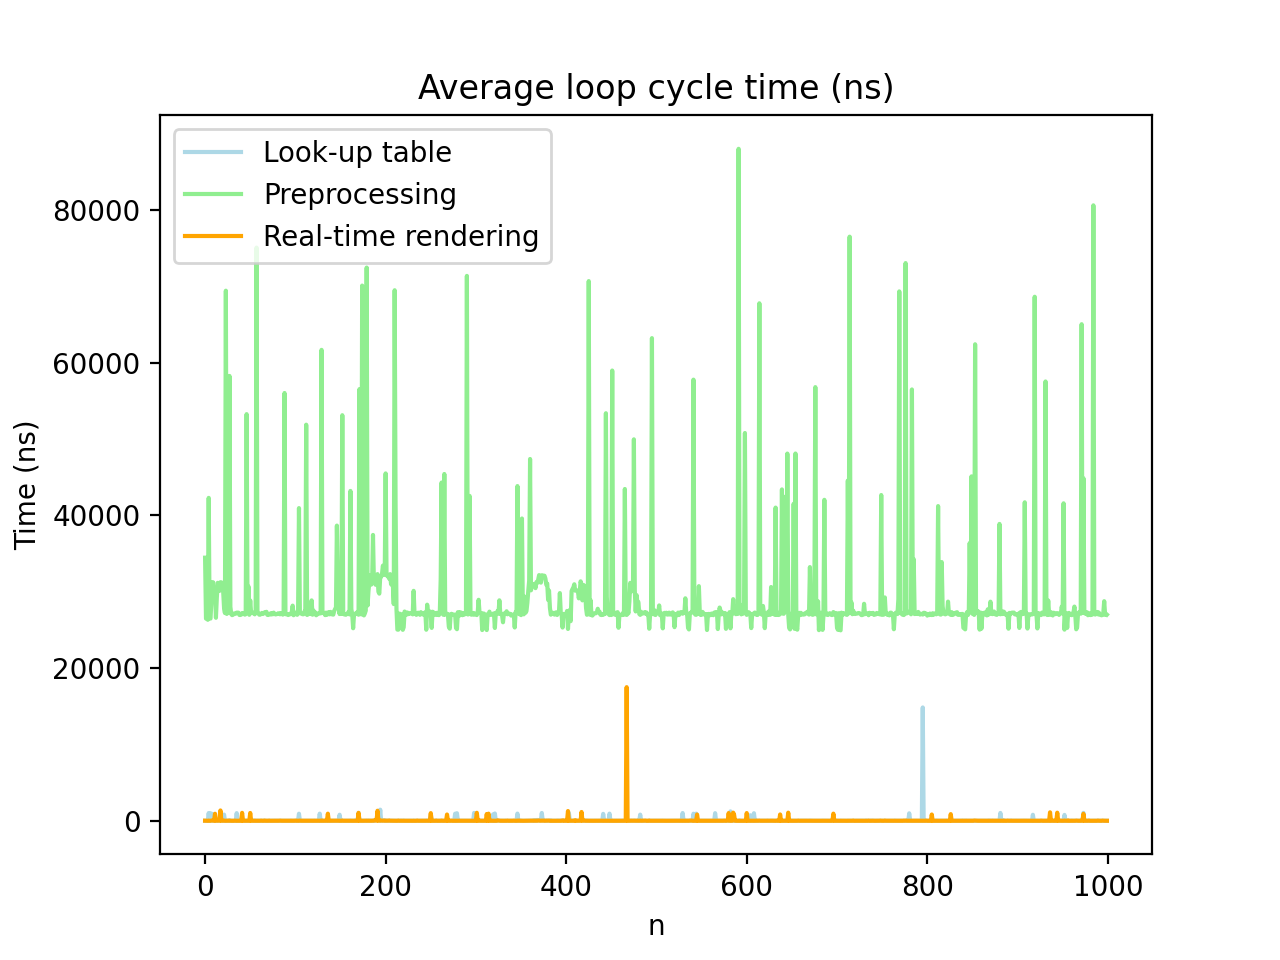
\includegraphics[width=\linewidth]{env_init_time.png}
	\caption{Initialization time, measured 1000 times.}
	\label{fig:env_init_time}
\end{figure}

The second graph, however, paints a different picture. Comparing the results in Figure \ref{fig:env_average_cycle_time}, both the pre-processing and real-time algorithm have an average render cycle time of around 42ns, while the look-up table method takes over 10ns longer. This puts especially the \textit{real-time rendering} method in a very good position, as it combines both a low average rendering time with an already fast initialization.
\begin{figure}[ht!]
	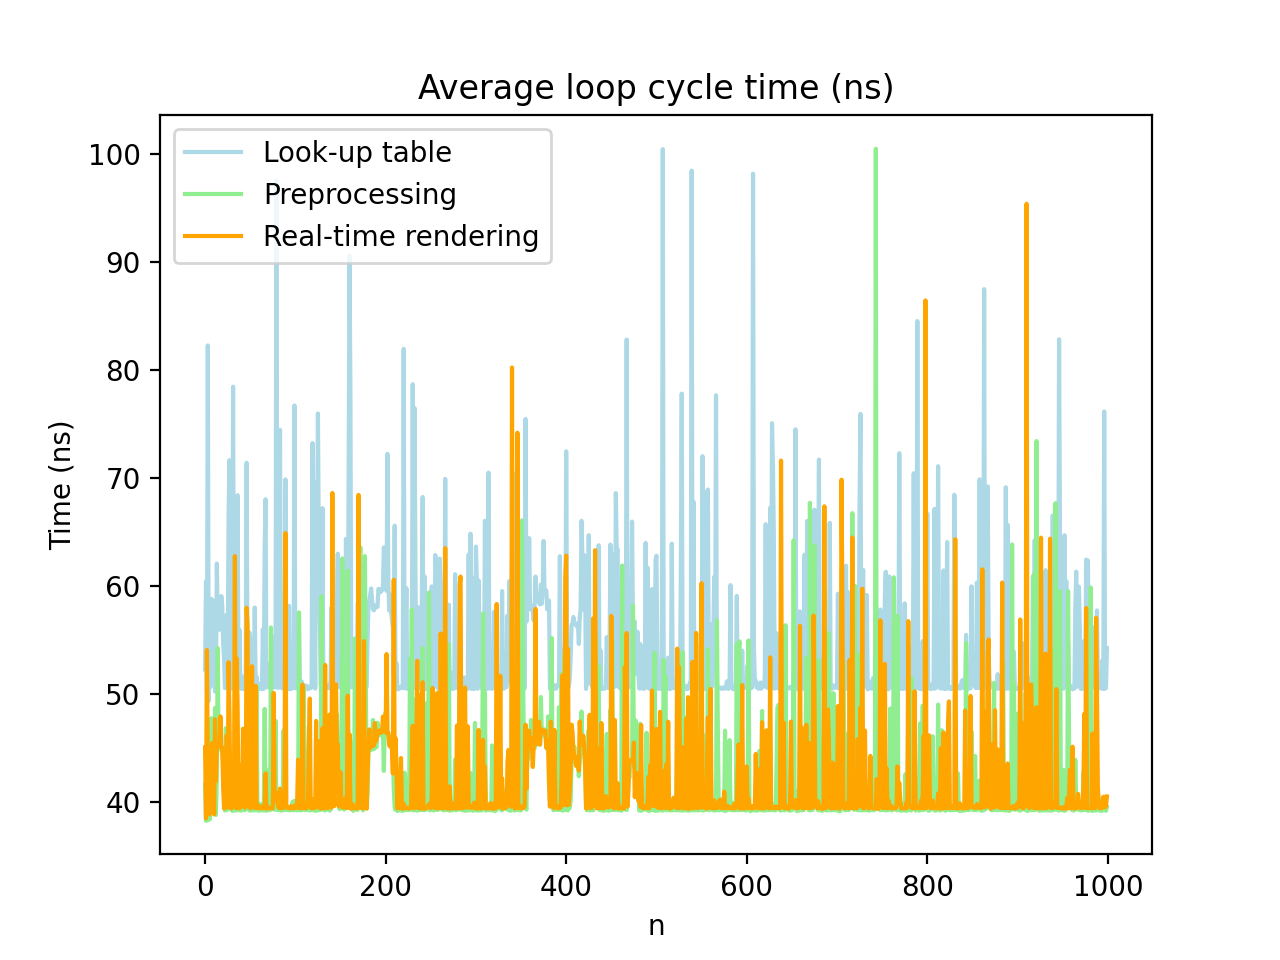
\includegraphics[width=\linewidth]{env_average_cycle_time.png}
	\caption{Average time per rendering cycle, measured 1000 times.}
	\label{fig:env_average_cycle_time}
\end{figure}

Finally, it may prove insightful to add some times together in order to provide a broad estimate of what rendering times for a complete granular implementation could look like. This does not reflect any additional processing such as filtering and recording, so one should take these results with a \textit{grain} of salt.\\
An example implementation using a \textit{divide-down} algorithm to schedule its grains and then applies an envelope using \textit{real-time rendering} will take approximately 450ns to complete. This accounts for about 2\% of the total available time. Another combination would add \textit{preprocessed} envelopes to a \textit{deterministic} scheduling approach, adding up to around 1.1$\mu$s and consuming about 4.7\% of the rendering cycle. As can be concluded from these two examples, a granular process like this should generally not add a big overhead to an audio rendering process.

\section*{Conclusions}
Over the past 75 years, granular synthesis has developed itself from cutting edge physics theory to commonplace tool in a musician's workshop. Thanks to the findings of scientists like Dennis Gabor and the work of musicians like Curtis Roads, instrument makers have yet another flavor to liven up their creations. When put to the test, this technique has proven itself rather versatile in both its applications and performance. Its existing implementations range from VST instruments to hardware effects, and the number of up-and-coming producers and composers using the technology is growing by the day.\\
This writing only covered a small share of many possible approaches to implementing elements of this technique, and therefore should not be considered a definitive list of available methods. It can, however, serve as the basis for new ideas and inspire completely new applications and implementations. The research has been done, the code has been written, and now it's time to play.

\printbibliography
\textit{All graphics in this writing were created by the author, unless otherwise noted.}

\end{document}